\documentclass [10pt]{article}

\usepackage {amsmath}
\usepackage {amssymb}
\usepackage {mathtools}
\usepackage {bbold}
\usepackage {multicol}
\usepackage [a4paper, total={16cm, 24cm}]{geometry}
\usepackage {titlesec}
\usepackage {enumitem}
\usepackage {csquotes}
\usepackage {graphicx}
\usepackage {caption}
\usepackage {tikz}
\usetikzlibrary {quantikz}

\renewcommand {\thesection} {\Roman{section}} 
\renewcommand {\thesubsection} {\thesection.\Roman{subsection}}

\titleformat {\section}
  {\normalfont\normalsize\bfseries}{\thesection.}{1em}{}
\titleformat {\subsection}
  {\normalfont\normalsize\itshape}{\thesubsection.}{1em}{}
\titleformat {\subsubsection}
  {\normalfont\normalsize\itshape}{\thesubsubsection.}{1em}{}

\setlength {\columnsep}{0.5cm}

\DeclareMathOperator* {\argmin} {argmin}
\newcommand {\qvec}[1] {\vert #1 \rangle}
\newcommand {\qcovec}[1] {\langle #1 \vert}
\newcommand {\qeval}[1] {\langle #1 \rangle}
\newcommand {\qinner}[2] {\langle #1 \vert #2 \rangle}
\newcommand {\qouter}[2] {\qvec{#1} \qcovec{#2}}
\newcommand {\qnorm}[1] {\lVert #1 \rVert}


\title {
	{\Large Seminar: Advanced Topics in Quantum Computing \\}
	\vspace {0.4cm}
	On efficient encodings for QAOA \\
	solutions to vehicle routing problems
}
\author {Eben Jowie Haezer}
\date {\today}

\begin {document}
\vspace* {-1.8cm}
{\let \newpage \relax \maketitle}

\begin {abstract}
This report details recent advances in optimising computational resource usage
for variational quantum approaches, with an application to solving the vehicle
routing problem (VRP) and its variants. This set of problems is of significant
importance with regard to logistical applications in industry. The quantum
approximate optimisation algorithm (QAOA) can be used to perform combinatorial
optimisation on present day gate system quantum devices. In accordance with
hardware input constraints, the problem is formulated as a quadratic
unconstrained binary optimisation (QUBO), which is equivalent to finding the
ground state of the corresponding Ising Hamiltonian. The simplistic complete
encoding that occurs naturally due to the problem formulation is compared
against a more recently proposed minimal encoding, which is capable of scaling
computational resource consumption logarithmically to problem size. The
benefits and drawbacks as well as overall feasibility of this encoding are
explored and discussed.
\end {abstract}

\vspace {0.3cm}

\begin {multicols}{2}

% structure:
%
% i.	introduction
% ii.	vrp
% iii.	algorithms
% iv.	qubo
% v.	encoding schemes
% vi.	discussion
% vii.	conclusion
% viii.	appendix

\section {Introduction}
The Vehicle Routing Problem (VRP) is concerned with finding optimal routes
for vehicles to deliver goods to a set of customers with some geographical
distance between them. It is obvious that this type of problem has far
reaching practical applications in various contexts, in fact the need to find
a reasonable solution is almost ubiquitous when dealing with logistical
planning, for example to determine efficient road, rail, shipping, and air
routes for commercial or public interest.

VRP, being itself a more general version of the Travelling Salesman Problem
(TSP), is similarly an NP hard \cite{vrp} combinatorial optimisation problem
with a solution space scaling factorially in the number of customers, thus
finding the definitive optimal solution through brute force becomes very
rapidly intractable even for relatively small problem sizes. The most
effective classical algorithms to date employed in practice revolve around
heuristics and greedy methods, some notable examples being tabu search
\cite{tabusearch} and column generation \cite{colgen}, able to construct
routes within single digit percentage tolerances \cite{metaheuristic} for
problem instances with verifiable optimal solutions.

More recently, the noisy intermediate scale quantum (NISQ) era \cite{nisq} has
paved the way for the development of variational quantum algorithms alongside
the potent quantum annealing \cite{annealintro} method as a contender for
computing reliable and near optimal solutions to combinatorial optimisation
problems, exploiting the unique inherent property of quantum algorithms to
operate on the entire solution space at once, albeit incrementally and
probabilistically \cite{qcintro}.

Initial tests have shown some promise in applying these quantum algorithms
to the VRP against classical solvers, achieving comparable accuracy on
small problem instances \cite{cvrpanneal} \cite{effvrp}.
However, as quantum hardware continues to improve, it makes
sense to also look at utilising it as efficiently as possible. Solving VRP
naively using quantum methods maps one whole qubit to one classical variable
\cite{effvrp},
quickly exhausting the already limited computing resources when introducing
additional constraints such as vehicle capacity or time windows on larger
problem scales more commonly encountered in practical scenarios.

This report discusses recent research into an idea to mitigate this
uneconomical use of computing power through a more clever and refined 
encoding of the input problem, in order to achieve a logarithmic scaling of
resource consumption with respect to problem size.
Section II outlines a formal description of the VRP and some of its variants
modelled as a graph problem.
In section III, quantum methods and algorithms for NISQ era processors that
see use in combinatorial optimisation are briefly highlighted.
Section IV discusses the problem formulation. It explains the QUBO and
its usage as an input method to solving the VRP on quantum hardware, along
with its relationship to the Ising model and in particular the
Ising Hamiltonian. From this, a formulation for the VRP can be derived.
Section V details encoding approaches onto the quantum system and lists
benefits and drawbacks for each, with a focus on managing computational
resource demand.
Published experimental observations describing the impact of the encodings
are depicted and discussed in Section VI,
and the report concludes in Section VII.

\section {Vehicle Routing Problem}
The vehicle routing problem (VRP) is a generalisation of the perhaps more
well known Travelling Salesman Problem (TSP), itself building upon the
Hamiltonian cycle problem first proved NP hard by Karp \cite{karp21}. VRP seeks
the optimal route or routes for a number of vehicles to traverse in order to
deliver certain goods to customers in various locations \cite{vrpintro}.

The problem is modelled intuitively by a graph $G = (V, E)$
where each node or vertex $v_i \in V$ represents the location of a customer 
and each edge $(i, j) \in E$ connecting two vertices corresponds to a path
traversible by a delivery vehicle. $\qnorm{V} = N$ is then the number
of customers considered. Traversing an edge $(i, j)$ incurs
a cost represented by $c_{ij} \in \mathbb R_{\ge 0}$, of which the total
value summed up across the entire journey is to be optimised, ie. made as
small as possible. This cost may be set based on travel time, distance,
or other concerns with economic consequences.

For simplicity, one can assume $G$ is a complete graph. Those edges directly
connecting two nodes $(i, j) \in E$ that are absent in reality can be labelled
with an edge cost $c_{ij} = c_{i n_1} + ... + c_{n_m j}$ corresponding to
the most efficient path available between them. This preprocessing step does
not necessarily complicate matters, and classical algorithms exist for all
pairs shortest path with known polynomial runtime performance, such as
the Dijkstra algorithm \cite{dijkstra}. Note that constantly traversing these
newly constructed edges is likely to be inefficient, since the vehicle may as
well service all the intermediate nodes $n_1 ... n_m$ along the way instead
of skipping them entirely. Furthermore, each graph contains a designated node
$v_0 \in V$ known as the depot. Valid routes must always begin and end at the
depot. A valid route is then a tuple $r = (v_n, v_{n+1}, ..., v_m)$ s.t.
$v_n = v_m = v_0 \; \land \; \forall n. \; (v_n, v_{n+1}) \in E$.

\vspace {0.3cm}
\begin {center}
\begin {tikzpicture}
\filldraw[black] (0,0) circle (2pt) node[anchor=east]{depot $v_0$};
\draw (3, 1) circle (2pt) node[anchor=south]{$v_j$};
\draw (4, 2) circle (2pt) node[anchor=west]{\small[4, 6]};
\draw (4, -0.2) circle (2pt);
\draw (0.7, 0.5) circle (2pt) node[anchor=south]{$v_i$};
\draw (1.3, 2.5) circle (2pt) node[anchor=north]{\small$d_k{=}5$};
\draw (-1, 1.5) circle (2pt);
\draw (0.7, 0.5) -- node[above]{$c_{ij}$} (3, 1);
\end {tikzpicture}
\captionof {figure}	{
	An illustration of the VRP as a graph problem. The white nodes represent
	customers, optionally with a demand value $d_k$ or a time window interval.
	One aims to find the most efficient route or routes (represented by the
	cumulative edge cost $\sum{c_{ij}}$) that delivers to all customers and
	respects the problem constraints.
}
\end {center}
\vspace {0.3cm}

For a problem to be classified as VRP, it should fulfil at least the above
minimal constraints. However, additional constraints may be imposed as
needed to better reflect a practical use case at the expense of slightly
complicating the model. For example, the capacitated VRP or CVRP stipulates
a fixed upper bound on the carrying capacity of each vehicle leaving the
depot, where in most cases this value is consistent across all vehicles
\cite{cvrpanneal}.
Customers $v_i$ are then assigned a score $d_i \in \mathbb R_{\ge 0}$ 
reflecting their demand quantity. This introduces the complication of
optimising with demands and constrained capacity as well as edge cost, and
the ideal solution for a given graph will in all likelihood differ from the
simple VRP.

On the other hand, the VRP with time windows (VRPTW) introduces a secondary
time parameter. Customers $v_i$ are assigned a certain time window
$[t_i^0, t_i^f] \subseteq \mathbb R_{\ge 0}$ in which they expect a delivery
\cite{effvrp}.
For the depot $v_0$ this interval is $[0, \infty)$ for simplicity. Hence the
edge costs $c_{ij}$ may also represent travel time between two nodes in this
formulation, and the objective shifts to finding the optimal route that
serves all customers whilst respecting these time windows, or failing this
attempting to maximise the number of customers or total goods supplied.

\section {Quantum Optimisation}

\begin {figure*}
\centering
\begin {quantikz}
& \gate[3]{H^{\otimes m}} & \gate[3]{e^{-i \gamma_1 H_f}}
& \gate[3]{e^{-i \beta_1 H_x}} & \qw \ \ldots \
& \gate[3]{e^{-i \gamma_n H_f}} & \gate[3]{e^{-i \beta_n H_x}}
\slice{$\rvert \psi(\beta, \gamma) \rangle$}
& \meter{} \arrow[r] &
\\
&&&& \qw \ \ldots \ &&& \meter{} \arrow[r] &
\rstick{\small observe and \\ \small optimise \\ parameters}
\\
&&&& \qw \ \ldots \ &&& \meter{} \arrow[r] &
\\
&& \arrow[u] \gamma_1 & \arrow[u] \beta_1 & (\small \text{depth }n)
& \arrow[u] \gamma_n & \arrow[u] \beta_n &&
\end {quantikz}

\caption	{
	Sketch of the QAOA setup. The state is brought into uniform superposition
	after which the repeated and alternating (layered) application of rotation
	operators realises approximately the time evolution under the Hamiltonian
	$H = H_f + H_x$ according to \eqref{lieprod}. The result is measured in the
	$Z^{\otimes m}$ basis and the tunable parameters $\beta, \gamma$ that affect
	each QAOA layer are optimised classically for the next run.
}
\label {qaoacirc}
\end {figure*}

Traditionally, quantum solvers for combinatorial optimisation problems have
been implemented using the quantum annealing approach \cite{annealising}
\cite{annealspinglass}. This method relies on the theory of adiabatic quantum
computation \cite{adiabaticsat} to evolve an easily prepared
ground state of the driver Hamiltonian $H_0$ gradually towards the ground state
of the problem Hamiltonian $H_p$. With sufficiently slow time evolution and
noncommuting Hamiltonians $[H_0, H_p] \neq 0$ (see Appendix \ref{adiabatic}),
the system is guaranteed to arrive in the desired ground state of the problem
by the adiabatic theorem \cite{adiabatictheo}.

More precisely, the system evolves according to
\begin {equation}
H(t) = \left(1 - \frac{t}{T}\right) \cdot H_0 + \frac{t}{T} \cdot H_p
\end {equation}
with $0 \leq t \leq T$, where the total algorithm runtime $T$ is bound by
$T \in \mathcal{O}(\frac{1}{g^2})$. Here $g$ denotes the spectral gap of $H$,
the minimal energy difference between the ground state and first excited
state throughout the evolution \cite{spectralgap}. Consequently, Hamiltonians
with narrower spectral gaps have to be evolved more slowly to prevent
excitation to the next energy level.

On the other hand, the more common circuit model processor operates based on a
series of quantum gates in a circuit. These gates are representative of a
limited set of unitary operators that are achievable on a chosen hardware
implementation. \cite{qcintro}. This principle of operation
is founded upon the solution to the time dependent Schrödinger equation for time
invariant Hamiltonians:
\begin {equation}
i \hbar \frac{\partial}{\partial t} \qvec{\psi(t)} = H \qvec{\psi(t)}
\Longleftrightarrow
U(t) = e^{\frac{-i}{\hbar}Ht}
\end {equation}
where $U$ denotes the unitary time evolution operator
(see Appendix \ref{schrodinger}), which may be decomposed into a series of
quantum gates. The quantum circuit thus realises the time evolution as
determined by the chosen Hamiltonian.

For Hamiltonians of the form $H = \sum_k H_k$, the following limit
equation \cite{matexp}, known as the Lie product formula or alternatively as
the Suzuki-Trotter expansion of the first order, provides a key insight for
$A, B \in \mathbb C^{m \times m}, m \in \mathbb N$:
\begin {equation}
\label {lieprod}
e^{A+B} = \lim_{n \rightarrow \infty}
\big(e^{\frac{A}{n}} \cdot e^{\frac{B}{n}}\big)^n
\end {equation}

As a result, the time evolution can be approximated as:
\begin {equation}
\label {unitaryiter}
U(t, n) = \prod_{j \le n} \prod_k \; e^{\frac{-i H_k t}{n}}
\end {equation}
ie. a series of smaller gate unitaries that may be repeated ad infinitum.

The advances in circuit model quantum processors that have brought
about the NISQ era have offered an alternative approach to tackle optimisation
problems, namely that of supplementing a quantum algorithm with classically
tuned parameters to iteratively arrive at a good approximation of the ground
state, known as hybrid algorithms \cite{variational}. NISQ era processors
are characterised \cite{nisq} by the primary limitation of restricted circuit
depth due to their limited coherence times and lack of fault tolerance.
These practical limitations prevent the use of high values of $n$ in
\eqref{lieprod}. However, by offloading some of the computation to a classical
algorithm and proceeding with iterative refinement, one can obtain reasonable
estimations of the ideal solutions to optimisation problems \cite{nisqalg}.

Following the recipe in \eqref{lieprod}, a circuit as in Fig.
\ref{qaoacirc}) is constructed out of alternating operators $H_f$ and $H_x$,
where the former represents the objective function and the latter is termed
a mixer Hamiltonian. Those variational approaches specifically intended for
combinatorial optimisation are given the name quantum approximate optimisation
algorithm (QAOA), first described by Farhi et al. in \cite{qaoaintro}.
\begin {equation}
\label {qaoa}
\qvec{\psi(\beta, \gamma)} =
\big( \prod_k e^{-i \beta_k H_x} e^{-i \gamma_k H_f} \big)
\; \qvec{+}^{\otimes m}
\end {equation}
Here $\qvec{+}^{\otimes m}$ is the uniform superposition obtained through
the Hadamard transform of the initial ground state, so as to begin optimising
from a neutral position where all possible solutions are considered.

The series of unitary evolutions are commonly implemented in the gate model as
qubit rotation operator arrays \cite{effvrp}. The parameters $\beta_i$ and
$\gamma_i$ represent angle values for these rotations $H_x$ and $H_f$
respectively, which can be interpreted as the discretised duration of time the
system spends under a particular unitary evolution due to \eqref{unitaryiter}.

Since $H_f$ is typically diagonal w.r.t. $Z^{\otimes n}$ (see below
\eqref{hdiag}), we typically choose the noncommuting mixer
$H_x = \sum_k \sigma^x_k$, also known as the transverse field mixer
(cf. \eqref{isingq}). However, this choice is by
no means inconsequential. Further studies have yielded more optimal choices for
$H_x$ and the initial system state tailored to the problem at hand, which allow
for overall quicker convergence to the optimum \cite{mixeropt}.

In any case, the primary purpose of the mixer is to allow the system to
escape undesirable local eigenstates in the course of running the algorithm.
For this, the noncommutative relation between the two operators ensures that
their individual eigenstates do not coincide (see Appendix \ref{adiabatic}).
From a macroscopic standpoint, the mixer acts to dissuade convergence towards
local minima by effectively reshuffling the state to an extent.

After performing the time evolution, the output state should attain increased
overlap to the desirable eigenstate. This more optimised result is read out with
high probability through a measurement and a classical optimiser attempts to
refine the angle parameters $\beta_i, \gamma_i$ for the next pass. The entire
procedure is then repeated until a sufficiently good solution is found. By the
adiabatic theorem and \eqref{lieprod}, arbitrarily precise solutions are
theoretically possible. In practice studies have highlighted certain limitations,
for example correlating solution quality inversely with the ratio of constraints
to variables in a problem \cite{qaoadensitybound}.


\section {Problem Formulation}
The quadratic unconstrained binary optimisation (QUBO) is concerned with
finding a binary vector $\qvec{x^*} \in \{0, 1\}^n$, $n \in \mathbb N$ that
fulfils the following optimal condition:
\begin {equation}
\qvec{x^*} = \argmin_{\qvec{x} \in \{0, 1\}^n} \; \qcovec{x} Q \qvec{x}
\end {equation}
where the linear operator $Q \in \mathbb R^{n \times n}$ is a symmetric
matrix. This can be interpreted as an objective function:
\begin {equation}
\label {qubo}
f_Q(x) = \qcovec{x} Q \qvec{x} =
\sum_{i = 1}^n \sum_{j = i}^n Q_{ij} x_i x_j
\end {equation}

In general, QUBO is also NP hard due to the exponential scaling of the
solution space in $\qnorm{\{0, 1\}^n} \in \mathcal{O}(2^n)$ with respect
to the number of dimensions $n$. Crucially, a useful property of QUBO is its
flexibility. One is able to encode in $Q$ various problem constraints, such
as connectivity and edge weightings of graphs. Significant efforts have been
invested such that many combinatorial optimisation problems have conversions
into QUBO \cite{isingnp} \cite{tutqubo},
not least the VRP and its variants \cite {qubolist}. These conversions
are useful to establish a uniform problem description for solvers to work with,
however in the context of quantum solvers, they are further motivated by the 
equivalence between QUBO and the Hamiltonian of the Ising model for
ferromagnetism.

\vspace {0.3cm}
\begin {center}
\begin {tikzpicture}
%\draw (0, 0) circle (2pt);
%\draw (2, 0) circle (2pt);
%\draw (4, 0) circle (2pt);
%;
%\draw (1, 1) circle (2pt);
%\draw (3, 1) circle (2pt);
%\draw (5, 1) circle (2pt);
%;
%\draw (2, 2) circle (2pt);
%\draw (4, 2) circle (2pt);
%\draw (6, 2) circle (2pt);
%;
\draw[gray, dashed] (0, 0) -- (2, 0);
\draw[gray, dashed] (4, 0) -- (2, 0);
;
\draw[gray, dashed] (0, 0) -- (1, 1);
\draw[gray, dashed] (2, 0) -- (3, 1);
\draw[gray, dashed] (4, 0) -- (5, 1);
;
\draw[gray, dashed] (1, 1) -- (3, 1);
\draw[gray, dashed] (5, 1) -- (3, 1);
;
\draw[gray, dashed] (1, 1) -- (2, 2);
\draw[gray, dashed] (3, 1) -- (4, 2);
\draw[gray, dashed] (5, 1) -- (6, 2);
;
\draw[gray, dashed] (2, 2) -- (4, 2);
\draw[gray, dashed] (6, 2) -- (4, 2);
;
\draw[->] (0, -0.2) -- (0, 0.2);
\draw[->] (2, -0.2) -- (2, 0.2);
\draw[->] (4, 0.2) -- (4, -0.2);
;
\draw[->] (1, 1.2) -- (1, 0.8);
\draw[->] (3, 1.2) -- (3, 0.8);
\draw[->] (5, 0.8) -- (5, 1.2);
;
\draw[->] (2, 1.8) -- (2, 2.2);
\draw[->] (4, 1.8) -- (4, 2.2);
\draw[->] (6, 1.8) -- (6, 2.2);
;
\end {tikzpicture}

\captionof {figure}	{
	Lattice structure depicting the Ising model in two dimensions. At each
	lattice site $k \in \Lambda$ an arrow represents the atomic spin
	$\sigma_k \in \{-1, 1\}$ that influences the local dipole moment. Dashed
	lines are nearest neighbour interactions $J_{ij}$.
}
\end {center}
\vspace {0.3cm}

The Ising model describes a lattice structure $\Lambda$ in which each lattice
site houses a particle. The spin of each particle is represented by a discrete
variable $\sigma_i \in \{-1, 1\}$, $i \in \Lambda$. This spin value governs the
local magnetic moment of the particle (see Appendix \ref{ising}).
Neighbouring lattice sites $\qeval{i\;j}. \; i, j \in \Lambda$ influence each
other, termed nearest neighbour interactions, whose interaction strength is
represented by $J_{ij} \in \mathbb R$. Furthermore, one may consider the
influence of an external field $h_i$ at site $i \in \Lambda$, such that the
spin wants to align with this field. \cite{isingmodel}

Thus the Hamiltonian reads:
\begin {equation}
\label {isingspin}
H = - \sum_{\qeval{i\;j}} J_{ij} \sigma_i \sigma_j - \mu \sum_{i} h_i \sigma_i
\end {equation}
where $\mu$ is the magnetic moment.

Replacing $\sigma$ with the Pauli operators yields the
quantum mechanical description:
\begin {equation}
\label {isingq}
H = - \sum_{\qeval{i\;j}} J_{ij} \sigma_i^z \sigma_j^z
- \mu \sum_{i} h_i^z \sigma_i^z - \mu \sum_{i} h_i^x \sigma_i^x
\end {equation}
where the second term with $\sigma^z$ describes the external longitudinal
field, and the final term with $\sigma^x$ describes the transverse field per
lattice site.

Notably, the Ising model is typically simplified to exclude the transverse
field, resulting in a classical Hamiltonian where the constituent terms
commute ie. a diagonal operator in the $Z^{\otimes n}$ basis.
\begin {equation}
\label {hdiag}
H = \sum_{z \in \{0, 1\}^n} E_z \; \qouter{z}{z}
\end {equation}
This means the ground state $E_0$ is described by a corresponding eigenvector
$\qvec{\phi}$ with $\phi \in \{0, 1\}^n$, allowing for simple measurement to
obtain an eigenvalue mappable to a specific bit string solution.

Through the reversible transformation $\sigma \mapsto 2x - 1$, where
$x \in \{0, 1\}$ s.t. $-1 \mapsto 0$ and $1 \mapsto 1$, one obtains the
equivalent QUBO formulation for free \cite{tutqubo}, and hence optimising for
the ground state of the Ising Hamiltonian is equivalent to optimising the
QUBO objective function.

With this knowledge, one can formulate the VRP as follows. We define the
set of constraints that a valid solution must adhere to:
\begin {itemize}
\item[\textbf{once}] Each customer $v_i$ is visited exactly once, ie. at a
	particular time step $t$ along a particular route $r_j$.
\item[\textbf{step}] For each time step $t$, each vehicle is either at a
	customer node $v_i$ or at the depot $v_0$.
\end {itemize}

Additional constraints may be specified depending on the problem variant.
For CVRP the following is useful:
\begin {itemize}
\item[\textbf{cap}] All routes $\{r_i\}$ respect the maximum capacity
	$m \in \mathbb R$ of a vehicle.
\end {itemize}

A homogeneous fleet of vehicles is assumed. Note that for simplicity, we do
not distinguish between vehicles and routes, under the premise that each route
will be navigated by exactly one vehicle. As a result, the number of routes is
limited to the number of vehicles. Furthermore, some CVRP variants consider
multiple depot nodes \cite{mdvrp}. This variant will not be further
investigated here.

Let $x_{t, i}^r \in \{0, \; 1\}$ denote the assignment of the customer node
$v_i$ to be visited along route $r \in \mathbb N_0$ at time step
$t \in \mathbb N_0$.
The first two constraints can then be described mathematically as follows:

\begin {equation}
H_{\text{once}} = \sum_i \; (1 - \sum_{r, \; t} x_{t, i}^r)^2
\end {equation}

\begin {equation}
H_{\text{step}} = \sum_{r, \; t} \; (1 - \sum_i x_{t, i}^r)^2
\end {equation}

The idea is to coerce each squared term to evaluate to zero, implying each
inner summation should evaluate to one. To illustrate, consider for example
$H_{\text{step}}$ which encodes the constraint \textbf{step}. We sum over all
node indices $i$, such that for a given step $t$ along the route $r$,
precisely one customer node or the depot is assigned to the schedule. In
general, once a constraint is violated it follows that the calculation yields
a positive result, after which penalty values may be applied accordingly.

Encoding the constraint \textbf{cap} is a little more involved:
\begin {equation}
H_{\text{cap}} = \sum_r \big( m - (\Delta + \sum_{t, \; i} d_i x_{t, i}^r) \big) ^2
\end {equation}
where $d_i$ represents the demand score of node $v_i$ and
\begin {equation}
\Delta = \sum_{b=0}^{\lceil \log_2 1+m \rceil - 1} 2^b \; a_b^r
\end {equation}

While the principle remains identical to the first two constraints,
the additional term $\Delta$ in $H_{\text{cap}}$ is a result of \textbf{cap}
being somewhat more relaxed, in that any value
$\sum_{t, \; i} d_i x_{t, i}^r \leq m$
for the loading of the vehicle is acceptable, instead of a hard requirement.
This is conveyed through the auxiliary variables $a_b^r \in \{0, \; 1\}$,
which may be freely set to perfectly zero out unused vehicle capacity for the
route $r$. Intuitively, $\Delta$ represents the tolerable deviation of the
amount loaded onto the vehicle on route $r$ compared to maximum capacity.
Naturally not fully loading the vehicle and forcing an early return to depot
may be suboptimal in many cases, however the edge cost metric represented by
the objective function $H_c$ should be sufficient to deter this.

\begin {equation}
H_c = \sum_{i, \; j, \; t, \; r} c_{ij} \; x_{i, t}^r \; x_{j, t+1}^r
\end {equation}

Coupled with the objective function given by $H_c$, the complete CVRP
Hamiltonian is the linear combination of these constraints:
\begin {equation}
\label {hcvrp}
H_p = H_c + p_1 H_{\text{once}} + p_2 H_{\text{step}} + p_3 H_{\text{cap}}
\end {equation}
Here $p_k \in \mathbb R_{\ge 0}$ with $k \in \{1, 2, 3\}$ corresponds to a
large penalty value that serves to mark a potential solution as undesirable,
in the case that one or more of the corresponding constraints are violated.
The exact values of $p_k$ are dependent on the problem instance and must be
heuristically determined and optimised \cite{cvrpqaoa} \cite{cvrpanneal}.

Crucially, this description of the CVRP is only one of several possible
formulations \cite{cvrpanneal}. Extensive research has been conducted into
determining the most optimal description that benefits solution quality as well
as speed of convergence. In particular, the formulation in \eqref{hcvrp} turns
out not to be suitable with regard to current limitations of NISQ era
processors, due to the large amount of free binary variables and comparative
lack of computing resources available to account for them all.

As it stands, the number of binary variables needed is in the order of
$\mathcal{O}(\qnorm{V}^3)$, considering the number of customer nodes, time
steps required, and routes or vehicles. One solution employed by
\cite{cvrpanneal} and \cite{cvrpqaoa} involves splitting the problem
into two distinct phases, a clustering phase that groups customer nodes
together similar to the knapsack problem, and a routing phase to determine the
ideal route in each of these clusters as in the TSP.

\vspace {0.3cm}
\begin {center}
\begin {tikzpicture}
\draw[magenta, style=dashed] (0, 0) -- (3, 1) -- (4.1, 1.2) -- (2.4, 0.1)
-- (0, 0);
\draw[cyan, style=dashed] (0, 0) -- (-1, 2) -- (1.3, 1.9) -- (3.5, 2.2)
-- (0.7, 0.5) -- (0, 0);

\filldraw[black] (0, 0) circle (2pt) node[anchor=south]{\small $v_0$};
\filldraw[black] (0, 0) circle (2pt) node[anchor=north]{\small $m{=}9$};
\filldraw[red] (3, 1) circle (2pt) node[anchor=north]{4};
\filldraw[blue] (0.7, 0.5) circle (2pt) node[anchor=north]{1};
\filldraw[blue] (-1, 2) circle (2pt) node[anchor=north]{2};
\filldraw[blue] (3.5, 2.2) circle (2pt) node[anchor=north]{2};
\filldraw[blue] (1.3, 1.9) circle (2pt) node[anchor=north]{3};
\filldraw[red] (4.1, 1.2) circle (2pt) node[anchor=north]{3};
\filldraw[red] (2.4, 0.1) circle (2pt) node[anchor=north]{2};
\end {tikzpicture}

\captionof {figure}	{
	The clustering and routing phase. The clustering phase divides nodes into
	collections (shown in blue and red) where the total demand obtained 
	through summation of the individual demand scores shown under
	each node does not exceed the vehicle capacity (in this case $m = 9$),
	similar to the multiple knapsack problem. The routing phase involves
	optimising each route individually for minimal edge cost as a TSP.
}
\end {center}
\vspace {0.3cm}

The clustering phase aims to discern routes by grouping nodes together in such
a way that \textbf{once} and \textbf{cap} hold true for each cluster.
Furthermore, intuition suggests neighbouring nodes should not be split apart
but rather be assigned to the same cluster to minimise edge costs.
\begin {enumerate}[label=\textbf{cluster}, align=left]
\item The cumulative edge cost $c_{ij}$ between all pairs of
	nodes $(i, j)$ within a cluster should be minimal.
\end {enumerate}

This results in the following problem Hamiltonian:
\begin {equation}
H_{\text{kn}} = q_1 H_{\text{once}} + q_2 H_{\text{cap}}
+ q_3 H_{\text{cluster}} 
\end {equation}
with penalty values $q_i$, where $H_{\text{cluster}}$ is defined as:
\begin {equation}
H_{\text{cluster}} = \sum_r \sum_{i, \; j} c_{ij} \; x_i^r \; x_j^r
\end {equation}
and $x_i^r = \sum_t x_{i, t}^k$.

It is worth noting that the penalty value $q_3$ should be set more modestly in
comparison to the others, given that \textbf{cluster} is not a hard constraint
but rather a metric measuring the optimality of clusters. It should always be
more appealing to relax \textbf{cluster} over violating $\textbf{once}$ or
$\textbf{cap}$ \cite{cvrpqaoa}.

Unfortunately, quantum solvers have been shown to perform relatively poorly 
when applied to the multiple knapsack problem \cite{multknapsack}, citing the
inefficiency brought about by having to invest qubits into encoding the free
binary variables $a_b^r$ for the constraint \textbf{cap}. Hence, at present,
the clustering phase should be deferred to a classical algorithm as
suggested in \cite{cvrpanneal}.

The routing phase takes the partitioned clusters and determines the optimal
route for each cluster locally. The problem is thus reduced to the TSP, which
conveniently has a QUBO formulation given in \cite{isingnp} as follows
\begin {equation}
H_{\text{tsp}} = q_1 H_{\text{once}} + q_2 H_{\text{step}} + q_3 H_c
\end {equation}
with the exception that, as we have broken up the problem and there is locally
only one route to optimise, in all terms we do not sum over $r$.

Overall, the TSP requires $\mathcal{O}(\qnorm{V}^2)$ binary variables to account
for all possible nodes and all possible time steps. Here \cite{isingnp} suggests
a resource optimisation saving to $(\qnorm{V} - 1)^2$ variables by fixing the
start node to be the depot $v_0$.



\section {Encoding Approaches}
We assume the use of a conventional NISQ processor to tackle a VRP involving
$n_c$ classical binary variables. A simple mapping from the VRP to QUBO uses
what is known as the complete encoding, where each classical binary variable
is represented by a single qubit, meaning each basis state corresponds to a
complete potential solution to the problem. The quantum state takes the form:
\begin {align}
\qvec{\psi(\theta)} 
&= U(\theta)\qvec{\psi_0} \\
&= \sum_{z \in \{0, \; 1\}^{n_c}} \alpha_z \qvec{z}
\end {align}

In this case, sampling the quantum state yields any given bitstring solution
${z \in \{0, 1\}^{n_c}}$ with probability $\qnorm{\alpha_z}^2$, where
$\alpha$ is parametrised by a set of angles $\theta$. In variational
algorithms, $\theta$ are heuristically determined values that serve to tune
arrays of rotation unitaries, which are adjusted after each pass to attain
the optimised state $\qvec{\psi^*} = U(\theta^*)\qvec{\psi_0}$
(cf. \eqref{qaoa}) \cite{qaoaintro}.

The QUBO objective function in the complete encoding is described by the
expectation of the equivalent Ising Hamiltonian:
\begin {equation}
C_{\text{cpl}}(\theta) = \qeval{H} = \qcovec{\psi(\theta)} H \qvec{\psi(\theta)}
\end {equation}


The advantage of the complete encoding is its ability to capture all
possible correlations between classical variables. This however sacrifices
scalability, requiring computational resources that scale proportionally
to the problem size as each binary classical variable is mapped to a
single qubit, hence $n_q = n_c$. As a result, feasible applications of the
complete encoding are limited to toy examples. Even as quantum hardware
becomes more powerful, it is prudent to examine encoding schemes that can more
efficiently take advantage of the available technology.

We consider the minimal encoding as presented in \cite{effbinopt}. This scheme
allows for $n_c$ classical variables to be mapped to $n_q = 1 + \log_2 n_c$
qubits, using a $n_r = \log_2 n_c$ wide register and $n_a = 1$ auxiliary
qubit.

Let $\{\qvec{\phi_i}\}$ and $\{\qvec{0}, \qvec{1}\}$ denote a basis for the
register and auxiliary qubits respectively. The system state $\qvec{\psi}$ is
then defined as:
\begin {equation}
\qvec{\psi(\theta)} = \sum_{i=1}^{n_c} \beta_i
(a_i \qvec{0} + b_i \qvec{1}) \; \qvec{\phi_i}
\end {equation}
where the coefficients $\beta_i$, $a_i$, $b_i$ are parametrised by $\theta$,
as in the complete encoding.

This encodes in the register the probability $\beta_i$ of measuring each
register state $\qvec{\phi_i}$ that corresponds to an individual classical
variable $x_i$, and in the auxiliary the probability of each of these binary
variables taking on the value $0$ or $1$ according to the Born rule:
$\Pr \; (x_i = 0) = \qnorm{a_i}^2$ and $\Pr \; (x_i = 1) = \qnorm{b_i}^2$.
Taken together, the probability of measuring a certain bitstring solution
$x$ for a given $\theta$ is expressed by:
\begin {equation}
\label {prob}
\Pr x = \prod_{i=1}^{n_c} \Pr x_i = \prod_{i=1}^{n_c} \qnorm{b_i}^2
\end {equation}

For example, consider $n_c = 4$, $n_r = 2$. The normalised system
state representing a particular bitstring $x^* = (1, 1, 1, 0)^\dag$
would be $\qvec{\psi^*} = \frac{1}{2}(\qvec{1}\qvec{00} + \qvec{1}\qvec{01}
+ \qvec{1}\qvec{10} + \qvec{0}\qvec{11})$.

The variational algorithm is run for several trials to obtain an estimate
of the coefficients $a_i$ and $b_i$, from which the probability distribution
for bitstring solutions as given in \eqref{prob} may be constructed.

With the minimal encoding a logarithmic scaling of qubits to classical
variables is achieved. However, this comes at the expense of a more limited
expressiveness in the quantum state. As seen in \eqref{prob}, the probability
distribution is sufficient to encode only statistically independent classical
variables, ie. those s.t.
$\forall i \; j. \; \Pr \; (x_i \land x_j) = \Pr x_i \Pr x_j$, which tend
not to be the case for highly complex and intertwined problems as in the VRP.
To illustrate, consider two nodes that both have a very high edge cost
connecting them to other nodes and the depot, but a negligible edge cost
between themselves. It is much more likely for these nodes to be visited
sequentially along a route, and hence the probability of visiting any one of
these nodes is greatly affected by whether its neighbour was visited at the
previous time step.

Reference \cite{effbinopt} claims this limitation is enough to limit quantum
advantage, to the point where classical simulations may actually be more
resource efficient. The independent probabilities governing the values of
binary classical variables may be simulated by as many classical continuous
variables \cite{contopt}.
Furthermore, the number of trials required to obtain a solution of
sufficient quality is necessarily increased, since utilising the register
addressing scheme for classical variables necessitates encoding them within a
superposition. Thereafter upon measurement, only the value of one classical
variable is obtained at a time. Depending on the exact problem
configuration, particularly small coefficient values in the quantum state
may result in certain bitstring outcomes being sampled too infrequently if at
all while evaluating the objective function, leading to inaccuracies. A
possible workaround for unsampled states is to assume $\Pr x_i = 0.5$ for an
unsampled classical binary variable $x_i$ as performed in \cite{effvrp},
though this is a very rough estimate at best.

Substituting \eqref{prob} into \eqref{qubo} and incorporating the
probabilistic component, we obtain the following objective function for the
minimal encoding:
\begin {align}
C_{\text{min}}(\theta)
&= \sum_{i \neq j}^{n_c} Q_{ij} \qnorm{b_i}^2 \qnorm{b_j}^2
+ \sum_{i=1}^{n_c} Q_{ii} \qnorm{b_i}^2 \\
&= \sum_{i \neq j}^{n_c} Q_{ij}
\frac{\qeval{P_i^1}}{\qeval{P_i}} \frac{\qeval{P_j^1}}{\qeval{P_j}}
+ \sum_{i=1}^{n_c} Q_{ii} \frac {\qeval{P_i^1}} {P_i}
\end {align}
expressed as projectors $P_i = \qouter{\phi_i}{\phi_i}$ and
$P_i^1 = \qouter{1}{1} \otimes P_i$.

Additionally, the minimal encoding scheme proposed here was originally
conceived for solving graph maximum cut problems \cite{effbinopt}. To this
end, the scheme can be extended to capture two body correlations, as opposed
to simply statistically independent variables as covered here. This proves
useful in the context of maximum cut, since one is interested in the
partitioning of nodes into two groups, and focuses on the edges connecting
the nodes. The ability to encode correlations in such a scheme also
allows quantum advantage to be retained.

The two body correlations were encoded as follows:
\begin {equation}
\begin {aligned}
\qvec{\psi(\theta)} = \sum_{i, \; j} \; \beta_{ij} \big(\alpha_{ij}^0 \qvec{00}
+ \alpha_{ij}^1 \qvec{01} \\ + \; \alpha_{ij}^2 \qvec{10}
+ \alpha_{ij}^3 \qvec{11} \big) \; \qvec{\phi_{ij}}
\end {aligned}
\end {equation}
While the overall scheme is similar, in this case the auxiliary is a $n_a = 2$
wide register which represents the values of pairs of binary variables
specified by the main register.

Reference \cite{effbinopt} further generalises the construction to encompass
many body correlations by way of subdividing binary variables into disjoint
sets and expanding the encoding accordingly, however with the drawbacks
of increased resource consumption and an increasingly difficult to compute
cost metric. The total number of qubits required is then given by
\begin {equation}
n_q = n_a + \log_2 \frac{n_c}{n_a}
\end {equation}
with the state then having the following representation:
\begin {equation}
\qvec{\psi(\theta)} = \sum_i \beta_i \; \big( \;
\sum_{\mathclap{z \in \{0, 1\}^{n_a}}} \; \alpha_i^z \qvec{z}
\big) \otimes \qvec{\phi_i}
\end {equation}
This results in $n_a$ groups of variables. The limiting case $n_a = n_c$ gives
the complete encoding. It remains to be seen whether VRP can better make use
of this, though this is unlikely given the interconnected nature of the problem.

What follows in the next section are experimental results from various
research papers analysing VRP solutions obtained through quantum algorithms on
NISQ era devices.
In order to examine the feasibility of the various encoding schemes for a
variety of problem sizes, we normalise the objective function in the following
manner:
\begin {equation}
C_{norm} = \frac{C(\theta) - C^*}{\Delta C}
\end {equation}
$C^*$ is the best known solution, typically as found by classical algorithms.
$\Delta C$ is the difference between $C^*$ and the worst case ie. maximal $C$.

\section {Experimental Results}
Reference \cite{effvrp} claims to have seen ideal convergence behaviour for
VRPTW with the minimal encoding for small scale problems, on occasion
surpassing that which was achieved when employing the traditional complete
encoding.

Figure \ref{2fig} depicts
how the optimiser iterations influenced the normalised cost compared to the
complete encoding for a VRP with $n_c = 16$. One observes the
expected reduction in solution quality using the minimal encoding, showing
more variance even with increased optimisation runs and requiring substantially
more sampling trials to get costs down.

\begin {center}
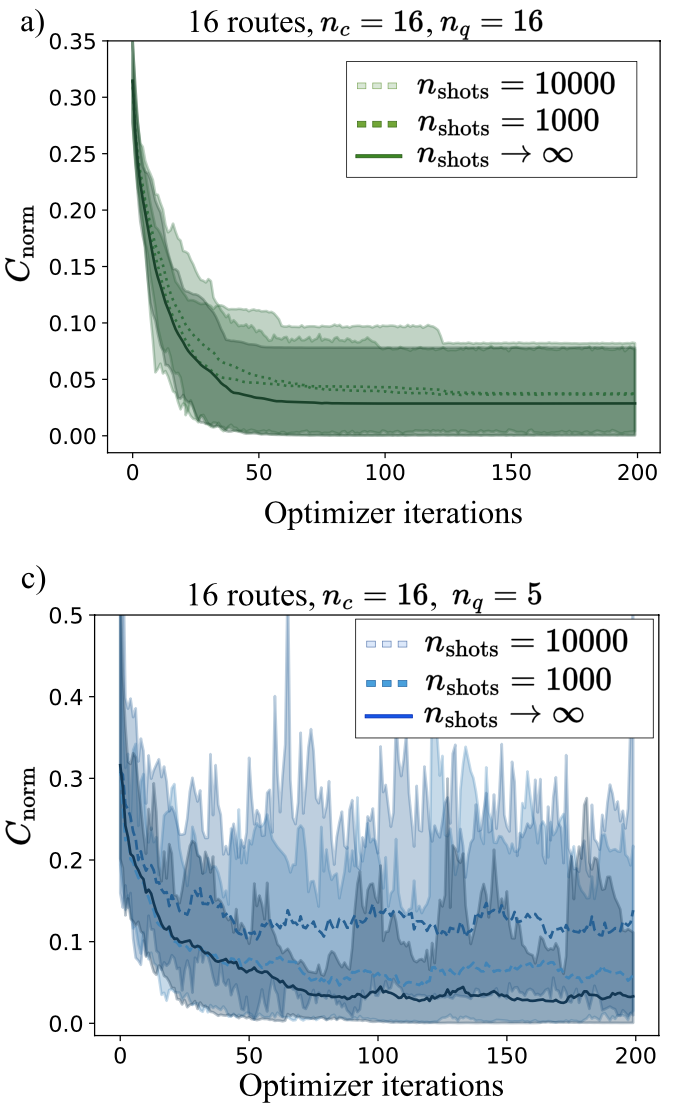
\includegraphics [width=\linewidth]{2fig}
\captionof {figure}	{
	Figure taken from \cite{effvrp}. Performance comparison between the
	complete encoding (a, top) and the minimal encoding (c, bottom) with
	respect to the solution improvement after several optimisation runs.
	$n_{\text{shots}}$ represents the curve obtained by sampling the state
	this many times. The limiting case is also shown. One observes markedly
	increased variance and slower convergence for the minimal encoding.
}
\label {2fig}
\end {center}

Meanwhile, Figure \ref{4fig} shows the cumulative distribution of solutions
obtained as a function of the normalised cost (labelled $C_{\text{norm}}$) on
several devices, plotted in colour. The black curve represents the distribution
of all possible solutions, or alternatively $4 \cdot 10^8$ randomly generated
solutions in cases where the former becomes too expensive to compute. A more
extreme gradient nearer the vertical axis, where the normalised cost is kept
at a minimum, reflects well on the overall procedure, as this means a higher
percentage of generated solutions are close to ideal.

\begin {figure*}[!ht]
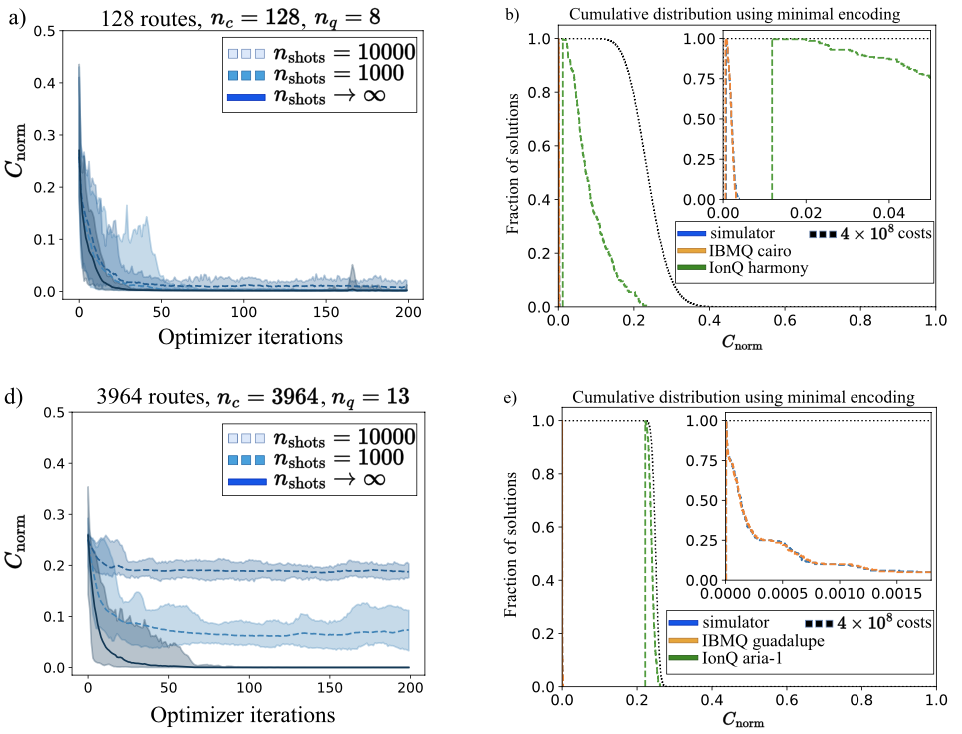
\includegraphics {4fig}
\caption	{
	Figure taken from \cite{effvrp}. The left column (a, d) shows optimisation
	runs with the minimal encoding for increasing problem sizes. Insufficient
	sampling led to convergence not being attained for $n_c = 3964$ classical
	variables. The right column (b, e) reflects the cumulative distribution of
	solutions obtained with the minimal encoding on various NISQ devices,
	compared with $4 \cdot 10^8$ randomly generated solutions charted in black.
}
\label {4fig}
\end {figure*}

Tests have also been conducted for larger problem instances that show
convergent behaviour, although sufficient iterations were not performed in
order for the convergence to manifest completely. This can be seen in
Figure \ref{4fig} (d), which for $n_c = 3964$ classical variables was still
a distance away from returning optimal solutions, limited by the relatively
modest count of 10000 sampling trials compared to $n_q = 13, 2^{n_q} = 8192$
different eigenstates. The authors of \cite{effvrp} assumed $p = 0.5$ for
unsampled variables and pointed to this as a reason for the suboptimal
convergence with increasing optimisation runs.

In comparison, \cite{cvrpqaoa} had notably worse results for the two phase
CVRP even for small problem sizes, using the complete encoding and QAOA to
optimise the routing phase as a TSP. However, they achieved significantly
better performance using a related variational algorithm termed variational
quantum eigensolver (VQE).

VQE normally sees use in similar optimisation problems in fields such as
quantum chemistry, again with the aim of finding the ground state of some
problem Hamiltonian. Unlike QAOA, VQE refines the initial state classically,
and formulates the problem Hamiltonian as a Pauli string $H = \bigotimes_i w_i
\cdot \{\mathbb{1}_i, \sigma^x_i, \sigma^y_i, \sigma^z_i\}$, and measures the
result in this manner as well \cite{vqe}.

In any case, the authors of \cite{cvrpqaoa} pointed to the problem formulation
as a factor that potentially inhibited the QAOA, and suggested an alternate
encoding might yield improved performance. Their attempt at solving the TSP
additionally tended to generate infeasible solutions, which did not correspond
to valid routes. Due to this, a large percentage of proposed solutions were of
little value and subsequently discarded. The researchers observed improvements
in the feasibility of returned solutions only as the approximated ground state
was within 97\% of the best known solution.

Based on these preliminary findings, it seems that the success that quantum
algorithms enjoy upon tackling VRP is heavily dependent on an advantageous
problem formulation. In light of this, continued research towards optimising
problem formulations for for various algorithms with an eye on resource
efficiency may yet prove fruitful as NISQ era processors become only more
potent with time.

\section {Conclusion}
The report summarises recent research into using quantum algorithms 
feasible on current NISQ era processors to derive approximate solutions to the
NP hard vehicle routing problem and its variants. Particular attention has been
drawn to the ways in which VRP can be cleverly formulated and encoded in order
to reduce the amount of computing resources required while still maintaining
an adequate solution quality.

Given the nature of quantum computation, the concept of employing it to deal
with complex and large scale search and optimisation problems will always be
appealing, especially once conventional classical methods reach their limits
of efficiency and accuracy as in the case of many NP problems. Although
classical solvers for VRP are for the moment still much more consistent and
yield more optimal results, research into quantum solvers may
yet provide valuable insight by demonstrating a different perspective in
tackling the problem. This research may additionally further the understanding
and improvement of the general implementation of successful quantum
optimisation, particulary the formulations and algorithms involved.

Present day hardware limitations in terms of scale and reliability remain a
significant hindrance in the pursuit of quantum advantage, hence the focus
of current research on  highly tunable hybrid variational algorithms. The
minimal encoding first described in \cite{effbinopt} uses logarithmically as
many qubits as classical binary variables in the problem, at the expense of
sacrificing the ability to encode correlations within variables. It has been
shown \cite{effvrp} to perform comparably to conventional encodings on both
small and large scales for certain problem formulations, highlighting that the
problem specifics greatly impact performance metrics, as is often the case
with quantum algorithms,

In the case of such a flexible problem as the VRP, ultimately the decision of
favouring one approach over another currently places a heavy emphasis on
experimental runs in order to determine their feasibilities for a particular
problem, as has been depicted in the results obtained above. Since this strong
dependency on the exact problem is well known, aside from looking into
alternative solution methods, a deeper analysis into the problem
characteristics that qualify a particular approach as suitable and developing
heuristics with which one is able to determine suitability may be a logical
next step.


\textit{Acknowledgements.}
This report was compiled as part of a quantum seminar held
at Technische Universität München during the 2023 winter semester. I would
like to thank Prof. Christian B. Mendl and my advisor Keefe Huang of the 
quantum research department at the university for their support in making
this project possible.

\bibliographystyle {IEEEtran}
\bibliography {report}

\appendix

\section {Schrödinger equation and unitarity}
\label {schrodinger}

Solving the time dependent Schrödinger equation for time invariant
Hamiltonians yields:
\begin {equation*}
\begin {aligned}
i \hbar \frac{\partial}{\partial t} \qvec{\psi(t)} &= H \qvec{\psi(t)} \\
i \hbar \; \frac{1}{\qvec{\psi(t)}} \; \partial \qvec{\psi(t)}
&= H \; \partial t \\
i \hbar \; \ln \frac{\qvec{\psi(t)}}{\qvec{\psi(t_0)}} &= Ht \\
\ln \frac{\qvec{\psi(t)}}{\qvec{\psi(t_0)}} &= \frac{-i}{\hbar}Ht \\
\qvec{\psi(t)} &= e^{\frac{-i}{\hbar}Ht} \qvec{\psi(t_0)} \\
\end {aligned}
\end {equation*}

Since $H$ is an observable describing the energy content of the system
eigenstates, it is Hermitian $H^\dag = H$ with real eigenvalues.
Hence:
\begin {equation*}
\begin {aligned}
U^\dag U &= (e^{\frac{-i}{\hbar}Ht})^\dag e^{\frac{-i}{\hbar}Ht} \\
&= e^{\frac{i}{\hbar}H^\dag t} e^{\frac{-i}{\hbar}Ht} \\
&= e^{\frac{i}{\hbar}Ht} e^{\frac{-i}{\hbar}Ht} \\
&= e^{\frac{i}{\hbar}(Ht - Ht)} \\
&= \mathbb{1}
\end {aligned}
\end {equation*}

In this manner the unitary time evolution preserves inner products, ie.
\begin {equation*}
\qinner{U\phi}{U\psi} = \qcovec{\phi} U^\dag U \qvec{\psi}
= \qinner{\phi}{\psi} 
\end {equation*}
for all $\qvec{\psi}, \qvec{\phi}$,
which in conjunction with the Born rule allows one to interpret the
wavefunction as a probability density.

\section {Commutativity and adiabatic theorem}
\label {adiabatic}
Commutativity in this case is defined through the Lie bracket operator
associated with the space of square matrices, ie. $[A, B] = AB - BA$.
Interpreted literally, it defines a metric describing whether the two matrices
$A$ and $B$ commute w.r.t. multiplication. $A$ and $B$ commute \textit{iff}
$[A, B] = 0$. Notably, two commuting Hamiltonians share an eigenbasis:
\begin {equation*}
A \qvec{\phi_i} = \lambda_i \qvec{\phi_i}
\end {equation*}
Hence:
\begin {equation*}
AB \qvec{\phi_i} = BA \qvec{\phi_i} = B \lambda_i \qvec{\phi_i}
= \lambda_i B \qvec{\phi_i}
\end {equation*}

The informal version of the adiabatic theorem is stated as follows:
\begin {displayquote}
\textit	{
A physical system remains in its instantaneous eigenstate if a given
perturbation is acting on it slowly enough and if there is a gap between the
eigenvalue and the rest of the Hamiltonian's spectrum. \cite{adiabatictheo}
}
\end {displayquote}

As such, in the case that the initial and final Hamiltonians $H_0$ and $H_p$
commute only the energies of the eigenstates are reassigned, and not the
eigenstates themselves. This runs the risk of equalising the energy levels of
the ground and excited states at some point during adiabatic evolution,
meaning the system is obliged to evolve infinitely slowly to obtain a
useful result due to $T \in \mathcal{O}(\frac{1}{g^2})$.

By the same reasoning, a noncommuting mixer is used in QAOA to allow
exploration of the search space by inducing transitions between eigenstates.

\section {Ising Model and Hamiltonian}
\label {ising}
Although the influence of a ferromagnetic particle is given as a magnetic
field that weakens over distance, it is sufficient to consider only nearest
neighbour interactions as a simplification.
The magnetic flux density for a dipole is
\begin {equation*}
\mathbf{B} = \frac{\mu_0}{4\pi} \; \big(\frac{3\mathbf{r(m \cdot r)}}{r^5}
- \frac{\mathbf{m}}{r^3}\big)
\end {equation*}
with $\mathbf{m}$ the magnetic moment \cite{dipoleflux}.
One observes from the first term that
for orientations orthogonal to the dipole the field strength drops off
substantially, and otherwise decays cubically with distance as given by the
second term. For an evenly spaced lattice any two particles have their influence
reduced by a factor of $\frac{1}{8}$ for each particle located in between them,
thereby justifying the nearest neighbour simplification.

When considering electrons, the spin is antiparallel to the magnetic moment,
given by an expression of this form:
\begin {equation*}
\mu = \frac{-e}{2m_e} L
\end {equation*}
where $L$ represents angular momentum \cite{mu_e}, so the Hamiltonian should be:
\begin {equation*}
H = - \sum_{\qeval{i\;j}} J_{ij} \sigma_i \sigma_j + \mu \sum_{i} h_i \sigma_i
\end {equation*}
however conventionally it is given as in (\ref{isingspin}), with the second term
carrying a negative sign \cite{isingconv}.

This results in the interactions being classified as ferromagnetic for
$J_{ij} > 0$ and antiferromagnetic for $J_{ij} < 0$.

\end {multicols}

\end {document}

